\clearpage
\appendix
\section{Derivation and Approximation Gap for $Y = X$}\label{appendix:allreduce-math}

This appendix derives the closed-form optimal partition $Y^*$ for R2CC-AllReduce and the approximation-gap bound for the $Y = X$ rule stated in Section~\ref{sec:single-failure}, then tabulates the actual per-$(n, X)$ gap values. Notation follows the main text: $D$ is the per-node data size, $B$ the per-node bandwidth, $n \geq 2$ the number of nodes, $X \in (0, 1)$ the bandwidth loss fraction on the failed node, and $Y \in [0, 1]$ the fraction of data routed through the partial AllReduce. The no-failure ring AllReduce time is $\frac{2(n-1)}{n} \cdot \frac{D}{B}$.

\paragraph{Stage times.} Stage 1 runs two AllReduces concurrently. The global AllReduce spans all $n$ nodes on $(1-Y)D$ and is bottlenecked by the failed node's $(1-X)B$:
$$T_1(Y) = \frac{2(n-1)}{n} \cdot \frac{(1-Y)D}{(1-X)B}.$$
The partial AllReduce involves the $n-1$ healthy nodes on $YD$ using their reserved $XB$:
$$T_2(Y) = \frac{2(n-2)}{n-1} \cdot \frac{YD}{XB}.$$
Stage 2 broadcasts the $YD$ partition back to the failed node, limited by its $(1-X)B$ receive bandwidth:
$$T_3(Y) = \frac{YD}{(1-X)B}.$$
The total completion time is $T(Y) = \max(T_1(Y), T_2(Y)) + T_3(Y)$.

\paragraph{Optimal partition.} $T_1$ strictly decreases and $T_2$ strictly increases in $Y$, so $\max(T_1, T_2)$ is minimized at the crossover $T_1(Y^*) = T_2(Y^*)$, giving
$$Y^* = \frac{(n-1)^2 X}{n^2 - 2n + X}.$$
For $Y \in [0, Y^*]$, $T(Y) = T_1(Y) + T_3(Y) = \frac{D}{nB(1-X)}\bigl[(-n+2)Y + (2n-2)\bigr]$ is non-increasing since $-(n-2) \leq 0$ for $n \geq 2$. For $Y \in (Y^*, 1]$, $T(Y) = T_2(Y) + T_3(Y) = YD\bigl[\frac{2(n-2)}{(n-1)XB} + \frac{1}{(1-X)B}\bigr]$ is strictly increasing. Therefore $T(Y) \geq T(Y^*)$ for all $Y \in [0, 1]$, so $Y^*$ is optimal. At $n = 2$ the coefficients degenerate and $T(Y)$ is constant, so the algorithm reduces to R2CC-Balance; for $n \geq 3$ the minimum at $Y^*$ is strict, and R2CC-AllReduce utilizes the $XB$ healthy-node bandwidth that would otherwise sit idle during the bottlenecked global ring.

\paragraph{Gap bound for $Y = X$.} Since $Y = X < Y^*$ lies in the non-increasing region $[0, Y^*]$ of $T(Y)$, algebra gives the closed form
$$g(n, X) := \frac{T(X) - T(Y^*)}{T(Y^*)} = \frac{Y^* - X}{\frac{2(n-1)}{n-2} - Y^*}.$$
Because $\frac{2(n-1)}{n-2} \geq 2$ for $n \geq 3$ and $Y^* < 1$, the denominator exceeds $1$, so the gap is strictly less than $Y^* - X$. Using the identity $Y^* - X = \frac{X(1-X)}{n(n-2) + X}$ together with $X(1-X) \leq 1/4$:
$$g(n, X) < Y^* - X \leq \frac{1}{4n(n-2)}.$$
At $n = 2$ the bound is vacuous because R2CC-AllReduce degenerates to R2CC-Balance.

Table~\ref{tab:approx-gap-max} lists $g(n, X)$ at three representative loss fractions $X \in \{1/8, 1/4, 1/2\}$ and three node scales $n \in \{4, 16, 64\}$, matching the $n$ values plotted in Figure~\ref{fig:appendix-approx-gap}. Even at $n = 4$ and the worst-case $X = 1/2$, the gap is only $1.19\%$; at $n = 16$ it is below $0.07\%$ across all three $X$, and at $n = 64$ it drops below $0.005\%$. $Y = X$ is therefore a near-optimal choice across all practical configurations.

\begin{table}[h]
\centering
\small
\begin{tabular}{rccc}
\toprule
$n$ & $X = \tfrac{1}{8}$ & $X = \tfrac{1}{4}$ & $X = \tfrac{1}{2}$ \\
\midrule
4 & $0.470\%$ & $0.833\%$ & $1.190\%$ \\
16 & $0.02419\%$ & $0.04419\%$ & $0.06783\%$ \\
64 & $0.00145\%$ & $0.00265\%$ & $0.00411\%$ \\
\bottomrule
\end{tabular}
\caption{Relative approximation gap $g(n, X) = (T(X) - T(Y^*))/T(Y^*)$ at representative $(n, X)$ values.}
\label{tab:approx-gap-max}
\end{table}

Figure~\ref{fig:appendix-approx-gap} plots $g(n, X)$ as a continuous function of $X$ for $n \in \{4, 16, 64\}$. Each $4\times$ increase in $n$ shifts the curve down by roughly $1.2$ decades on the log $y$-axis, matching the $1/n^2$ asymptotic decay.

\begin{figure}[t]
    \centering
    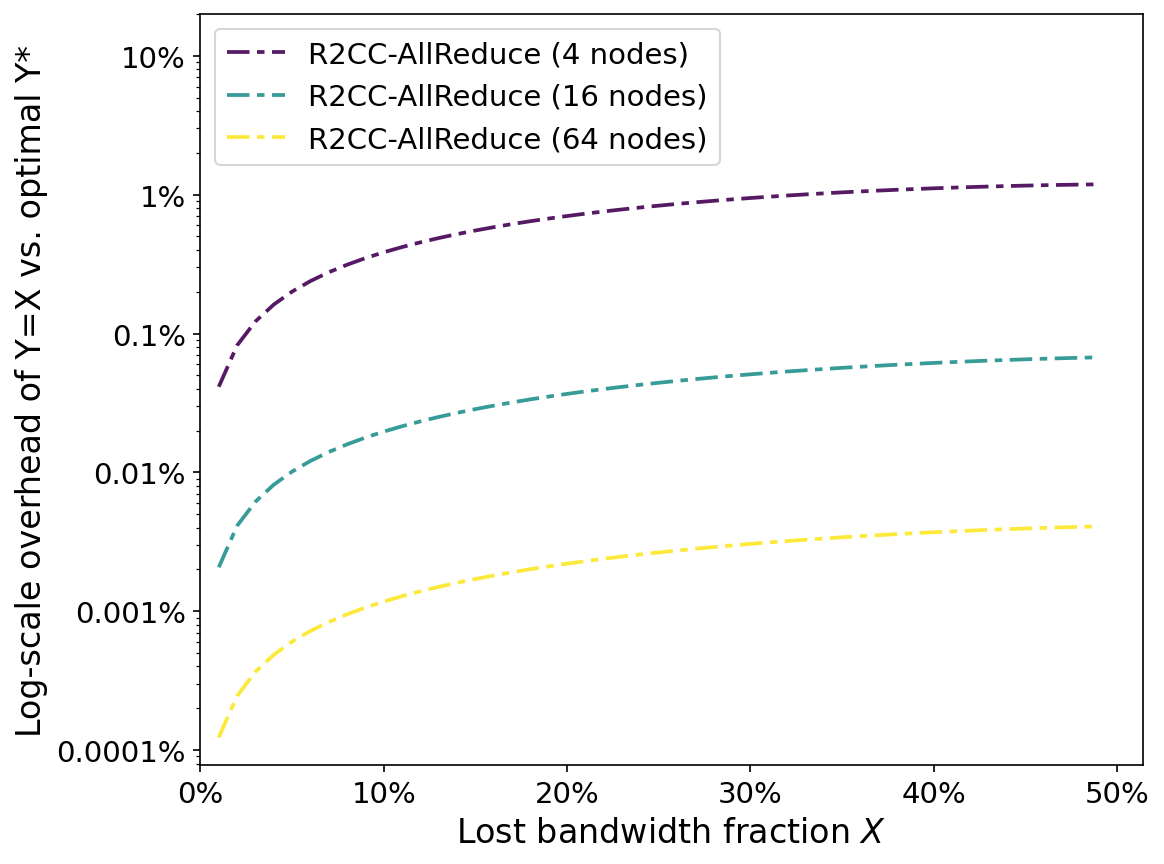
\includegraphics[width=0.9\columnwidth]{figs/approximate_gap.png}
    \tightcaption{Relative approximation gap $g(n, X) = (T(X) - T(Y^*))/T(Y^*)$ of the $Y = X$ rule vs.\ lost bandwidth fraction $X$, for $n \in \{4, 16, 64\}$. $y$-axis on log scale.}
    \label{fig:appendix-approx-gap}
\end{figure}

\section{Detailed Overhead Analysis}\label{appendix:overhead}

The overhead of using multiple NICs is confined to the I/O and host memory rather than to GPU memory or NVLink if using PCIe and QPI. When direct GPU–NIC access is available, R2CC registers the same GPU buffer with all NICs once at communicator creation and reuses this mapping for rerouted traffic, so no additional device memory is allocated. When a GPU–NIC pair cannot use direct access or cross NUMA, R2CC instead binds the collective to pinned host buffers and relies on CPU‑assisted copies, which likewise keep the GPU’s memory footprint unchanged. Prior work~\cite{liu2023hostping} shows that cross‑socket paths to a remote‑NUMA NIC can sustain more than half of the NIC’s line rate with only modest latency increase, which is sufficient to carry the fraction of traffic shifted off a failed NIC. When R2CC chooses PXN to avoid oversubscribed PCIe root complexes or CPU interconnects, the proxy GPU needs to allocate a small staging buffer on the order of tens of megabytes to relay segments to its local PCIe‑attached NIC, incurring one extra hop on NVLink but still negligible GPU‑memory overhead compared to model state.

\section{Detailed R2CC Failure Handling Scope}\label{app:failure-scope}

Table~\ref{tab:r2cc-failure-scope} summarizes R2CC's failure-handling scope, separating failures R2CC handles in-flight (fully or partially) from out-of-scope fundamentals that are left to higher-layer recovery.

\paragraph{Gray failures and link flapping.}\label{app:gray-failure}
R2CC detects failures through transport-level errors, such as work request completions that exceed the retry limit, and initiates recovery as described in \S\ref{sec:design-mig}. However, link flapping or packet loss masked by RDMA retransmissions does not produce such errors, leaving R2CC unaware of the degradation. Consequently, fault localization and HotRepair are not triggered, and collective operations continue to complete correctly, but at reduced throughput (Table~\ref{tab:r2cc-failure-scope}).
While detecting such gray failures is a limitation of the current design, R2CC-Balance (\S\ref{sec:single-failure}) already distributes traffic in proportion to per-NIC bandwidth. A possible extension would therefore be to use observed per-channel bandwidth to drive rebalancing, potentially mitigating gray failures that manifest as sustained throughput degradation.

\begin{table*}[!t]
\centering
\begin{tabular}{p{0.30\textwidth}p{0.12\textwidth}p{0.50\textwidth}}
\toprule
\textbf{Failure Type} & \textbf{Support} & \textbf{When Supported (Boundary)} \\
\midrule

\multicolumn{3}{l}{\textit{In-flight inter-node communication failures (R2CC’s primary scope)}} \\
\midrule
NIC hardware / port failure (incl. NIC--ToR) & Yes &
Node/process stays alive, and the node still has at least one remaining healthy inter-node NIC/path. \\
\addlinespace

Inter-node link / cable / ToR port down (single rail/link) & Yes &
An alternate inter-node path exists (e.g., another rail/NIC); not a full network partition. \\
\addlinespace

RDMA transport / QP-level failure (error CQE, QP error, WQE flush) & Yes &
Failure is confined to a subset of connections while endpoints remain alive and an alternate NIC/path exists. \\
\addlinespace

Link flapping (up$\rightarrow$down$\rightarrow$up) & Partial &
Only when flapping causes an in-flight transport failure (e.g. timeout) visible to the collective; pure throughput jitter is not handled. \\
\addlinespace

Multi-hop fabric fault (Inter-switch link / spine switch failure) & Partial &
Usually masked by fabric rerouting; if it surfaces as a transport error, handled via backup connections. \\
\addlinespace

CRC error (packet corruption) & Partial &
Only when CRC errors escalate into an in-flight transport failure; otherwise typically no recovery action is triggered. \\
\addlinespace

NIC driver issue & Partial &
Supported only if it does not crash the OS/process and still leaves an alternate NIC/path usable. \\
\addlinespace

NIC firmware issue & Partial &
Supported only if it degrades a subset of NICs while the node/process remains alive and other NICs/paths remain usable. \\
\addlinespace

PCIe failure (NIC unreachable / disappears) & Partial &
Supported when PCIe issues take down only a subset of NICs while other NICs remain usable; system-wide I/O failure is out of scope. \\
\addlinespace

GPU$\leftrightarrow$NIC direct path unavailable (GPUDirect / PCIe P2P degraded) & Partial &
Supported only if communication can continue via other usable inter-node NIC/path (potentially with degraded performance). \\

\midrule
\multicolumn{3}{l}{\textit{Out-of-scope fundamentals}} \\
\midrule

NVLink / NVSwitch failure (intra-node fabric) & No &
Not supported. \\
\addlinespace

Network partition / switch-wide outage (no alternate path) & No &
Not supported. \\
\addlinespace

Node/OS/process crash / GPU failure & No &
Not supported. \\
\addlinespace

Cross-rail mistaken wiring & No &
Out of scope; assumes the job can initialize and run normally. \\
\bottomrule
\end{tabular}
\caption{\textbf{R2CC failure model and scope.} Support means the system can keep an ongoing collective running without communicator re-initialization or job restart, under the stated boundary conditions.}
\label{tab:r2cc-failure-scope}
\end{table*}

\section{Optimize Scheduling Under Multi-Failure}
\label{sec:multi-failure}
Large-scale distributed GPU clusters can face concurrent failures~\cite{Revisiting_Reliability}.
Extending single-failure handling to support multi-failure resilience introduces two formidable challenges:
(1) Topological Fragmentation: In rail-optimized topologies, asymmetric failures on adjacent nodes (e.g., Node A loses NIC 1, while Node B loses NIC 2) disrupt the alignment of parallel rails, rendering simple local load balancing insufficient.
(2) Bandwidth Spectrum: Multiple failures create a spectrum of available bandwidth capacities across nodes, rather than a binary healthy/faulty distinction.
In this section, we present how R2CC generalizes its scheduling primitives to address these complexities through \textit{Topology-Aware Logical Re-ranking} and \textit{Recursive AllReduce Decomposition}.

\begin{figure}
    \centering
    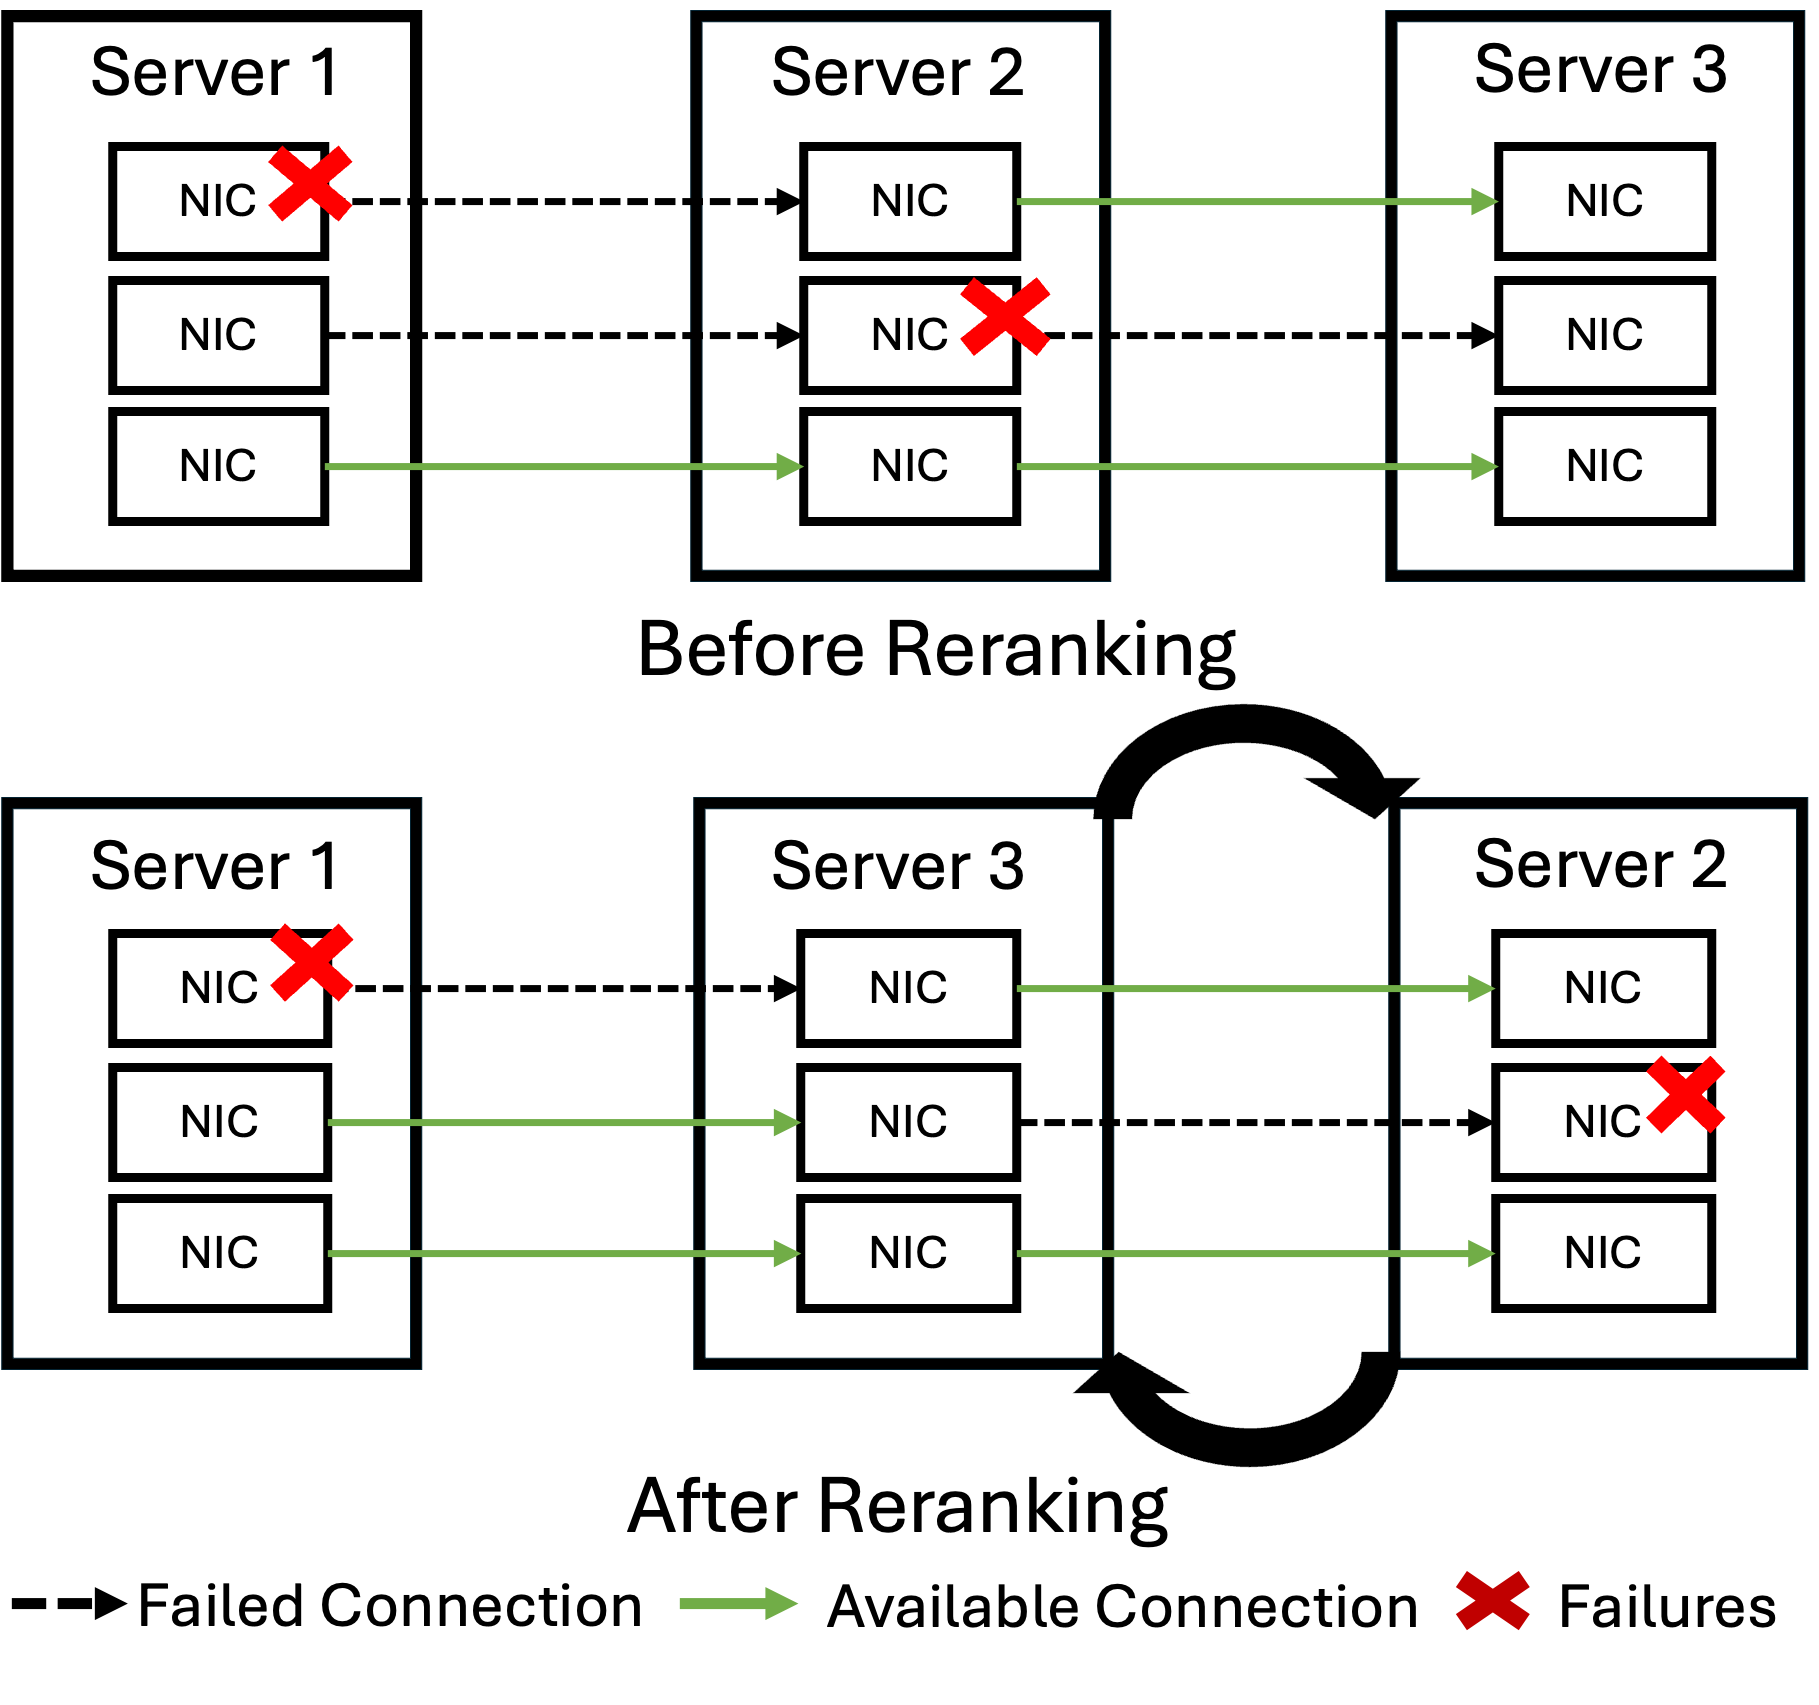
\includegraphics[width=0.7\columnwidth]{figs/design/figure6-1.png}
    \vspace{-5pt}
    \tightcaption{\textbf{Topology-aware logical re-ranking.}}
    \label{fig:Bandwidth Bridge}
\end{figure}

\paragraph{Topology-Aware Logical Re-ranking.} NCCL typically fixes ring/tree order by physical locality or static configuration. When adjacent nodes experience disjoint NIC failures (e.g., node $u$ loses rail $r$ while neighbor $v$ loses rail $r'$), their shared bandwidth drops to the narrow intersection of surviving rails, and local load balancing can no longer compensate.

We observe that most collective algorithms are symmetric and agnostic to node ordering, enabling safe reordering. It performs topology-aware logical re-ranking (Figure~\ref{fig:Bandwidth Bridge}): pairs of neighbors whose rail overlap falls below a bandwidth threshold are separated by inserting “bridge’’ nodes with broader rail connectivity. This targeted repair modifies only the problematic edges rather than rebuilding the entire ring, preserving most RDMA connections.

\paragraph{Recursive R2CC-AllReduce.} The R2CC-AllReduce strategy in Section~\ref{sec:single-failure} isolates a single bottleneck node and reduces its communication load, assuming the remaining nodes are homogeneous. Under concurrent failures, however, clusters develop a bandwidth spectrum, and treating all non-bottleneck nodes as a single group forces faster nodes to operate at the speed of moderately degraded ones, leaving substantial bandwidth unused.

R2CC addresses this by generalizing dual-ring decomposition into a recursive scheduling strategy. The system first forms a global ring running at the slowest node’s rate. It then isolates that node and builds a faster sub-ring from the remaining participants. If bandwidth variance persists, R2CC recursively peels off further sub-rings, each handling a data chunk proportional to the incremental bandwidth of its members. Logical re-ranking is applied at every level to avoid rail mismatches introduced by skipping slower nodes.

R2CC executes the reduction phases of all rings in parallel to saturate available bandwidth. Broadcast phases impose dependencies—slower nodes must wait for partial results from faster sub-rings—but bandwidth asymmetry often allows faster nodes to finish their smaller broadcasts concurrently with slower nodes' ongoing operations. To formalize these decisions, R2CC extends NCCL’s performance model ($\alpha$–$\beta$) to evaluate expected completion time at each recursion depth, incorporating per-node bandwidth and overlap. The planner then selects among standard Ring/Tree, R2CC-Balance, or recursive R2CC-AllReduce to best navigate latency–throughput trade-offs.

\paragraph{Severe single node and rail failures.} By the model of \S\ref{sec:single-failure}, losing 2 or 3 NICs on the same node ($X=1/4, 3/8$) slows each AllReduce by 17--22\% and 30--40\% with R2CC-AllReduce on 4--128 nodes, and by 33\% and 60\% with R2CC-Balance (table below). A ToR switch failure that takes out a full rail removes the same NIC from every node, leaving no spare bandwidth for R2CC-AllReduce, so R2CC-Balance operates at 14.3\% overhead for one of eight rails. End-to-end overheads are much smaller: on our testbed, two simultaneous NIC failures on one node add at most 1.01\% training overhead (\S\ref{exp:training}), and up to seven failed NICs on one node keep inference within about 5\% (Figure~\ref{fig:multi_failure}).

\begin{center}
\small
\setlength{\tabcolsep}{4pt}
\begin{tabular}{lcccccc}
\toprule
Failure & $X$ & Balance & $n{=}4$ & $16$ & $64$ & $128$ \\
\midrule
1 NIC, 1 node & $1/8$ & 14.3 & 9.5 & 7.6 & 7.3 & 7.2 \\
2 NICs, 1 node & $1/4$ & 33.3 & 22.2 & 17.8 & 16.9 & 16.8 \\
3 NICs, 1 node & $3/8$ & 60.0 & 40.0 & 32.0 & 30.5 & 30.2 \\
Full rail & $1/8$ & 14.3 & \multicolumn{4}{c}{no gain (same as Balance)} \\
\bottomrule
\end{tabular}
\end{center}

\section{R2CC Bridge-Based Re-ranking}
\label{app:bridge-based}

Algorithm~\ref{alg:reranking} inserts bridge nodes with broader rail connectivity between ring neighbors whose surviving rail overlap falls below the global bandwidth threshold, repairing only the problematic edges while leaving the rest of the ring intact.

\begin{algorithm}[t]
\small
\caption{R2CC Bridge-Based Re-ranking}
\label{alg:reranking}
\textbf{Input:} Logical Ring $R$, Rail Sets $S$ \\
\textbf{Output:} Optimized Ring $R'$
\begin{algorithmic}[1]
\STATE \textbf{Initialize} $R' \leftarrow R$, $Candidates \leftarrow \emptyset$
\STATE $B_{global} \leftarrow \min_{n \in R} |S_n|$
\FOR{$i \leftarrow 0$ \textbf{to} $|R| - 1$}
    \STATE $u \leftarrow R[i]$, $v \leftarrow R[(i+1) \pmod{|R|}]$
    \IF{$|S_u \cap S_v| < B_{global}$}
        \STATE $Candidates.\text{add}((u, v))$
    \ENDIF
\ENDFOR
\STATE \textbf{Sort} $Candidates$ by severity (gap size) descending
\FOR{each pair $(u, v)$ in $Candidates$}
    \STATE $BestBridge \leftarrow \text{None}$
    \FOR{each node $w \in R' \setminus \{u, v\}$}
        \STATE $x \leftarrow \text{PrevNode}(w), y \leftarrow \text{NextNode}(w)$
        \STATE $NewCap \leftarrow \min( |S_u \cap S_w|, |S_w \cap S_v| )$
        \STATE $RemovalCap \leftarrow |S_x \cap S_y|$
        \IF{$NewCap \ge B_{global}$ \textbf{and} $RemovalCap \ge B_{global}$}
             \STATE $BestBridge \leftarrow w$
             \STATE \textbf{break}
        \ENDIF
    \ENDFOR
    \IF{$BestBridge \neq \text{None}$}
        \STATE $R'$.Relocate($BestBridge$, between $u, v$)
    \ENDIF
\ENDFOR
\STATE \textbf{return} $R'$
\end{algorithmic}
\end{algorithm}

\begin{figure}[t]
    \centering
    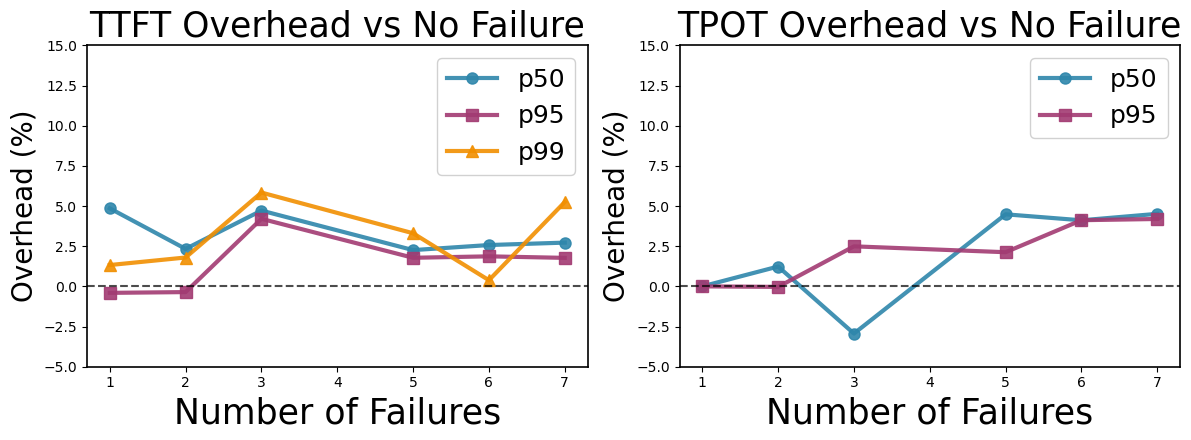
\includegraphics[width=1\linewidth]{figs/experiments/multi_failure.png}
    \caption{p50/p95 TTFT/TPOT overhead vs number of failures under multiple NIC failures for serving with pipeline parallelism}
    \label{fig:multi_failure}
\end{figure}

\section{Additional Evaluation Results}\label{appendix:collectives}

\paragraph{R2CC Inference Performance Under Multiple Failures.}\label{multi-failure-inference} We further evaluate R2CC's resilience under multiple concurrent failures on our two-node testbed. Unlike training workloads that may scale to hundreds of nodes, inference deployments typically use fewer nodes per model instance, reflecting production requirements for latency and cost efficiency. Our multi-failure experiments use vLLM engine to serve a 405B model with TP=8 and PP=2 configuration. We inject varying numbers of failures to reduce available NICs on a single node and feed requests at QPS=0.1, ensuring the system operates within its capacity to measure steady-state overhead. As shown in Figure \ref{fig:multi_failure}, both TTFT and TPOT overheads remain within 0-5\%, exhibiting minimal variance due to system underlying overhead, even as multiple network device failures reduce majority bandwidth. This demonstrates that R2CC fully exploits the ample bandwidth headroom in inference workloads: even under more severe and numerous failures on network devices, the remaining links still suffice to allow the system to continue serving with overhead close to zero.

\paragraph{Other Collective and Point-to-Point Operations.}
Beyond AllReduce, we evaluate R2CC-Balance on AllGather, ReduceScatter, and point-to-point (SendRecv) operations. Figure~\ref{appendix:fig:nccl-test-allreduce} shows that R2CC-Balance consistently maintains 83--90\% of normal throughput across these three operations for large messages, while the R2CC-HotRepair approach suffers approximately 50\% throughput loss due to its single-NIC bottleneck.

These results demonstrate that R2CC's load-balancing mechanism generalizes effectively beyond AllReduce, providing consistent fault tolerance for the full range of communication primitives used in modern distributed ML systems.

\begin{figure}
    \centering
    \begin{subfigure}[b]{0.48\columnwidth}
        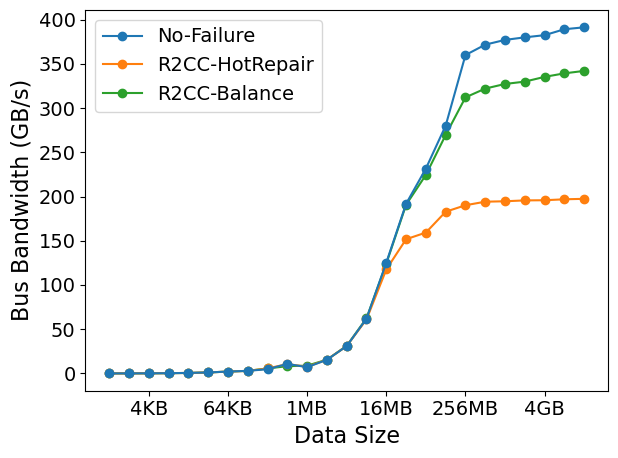
\includegraphics[width=\textwidth]{figs/section8/all_gather.png}
        \caption{AllGather}
        \label{fig:allgather-h100}
    \end{subfigure}

    \vskip\baselineskip

    \begin{subfigure}[b]{0.48\columnwidth}
        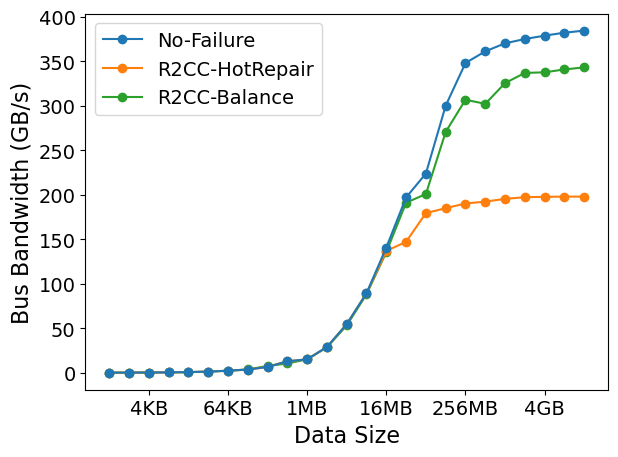
\includegraphics[width=\textwidth]{figs/section8/reduce_scatter.png}
        \caption{ReduceScatter}
        \label{fig:reducescatter-h100}
    \end{subfigure}
    \hfill
    \begin{subfigure}[b]{0.48\columnwidth}
        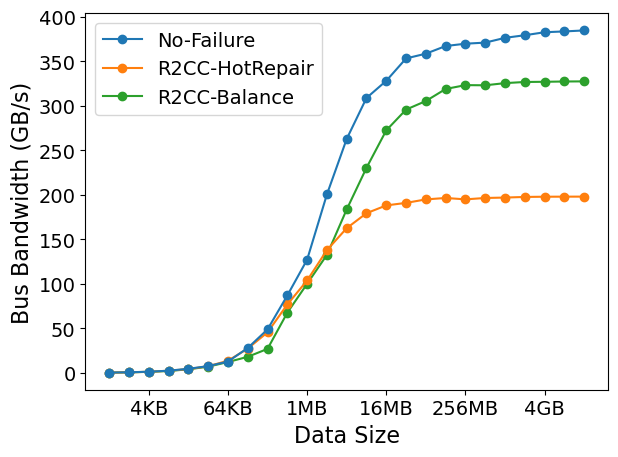
\includegraphics[width=\textwidth]{figs/section8/sendrecv.png}
        \caption{SendRecv}
        \label{fig:sendrecv-h100}
    \end{subfigure}

    \tightcaption{H100 NCCL-Test Benchmark.}
    \label{appendix:fig:nccl-test-allreduce}
\end{figure}
\begin{figure}
    \centering
    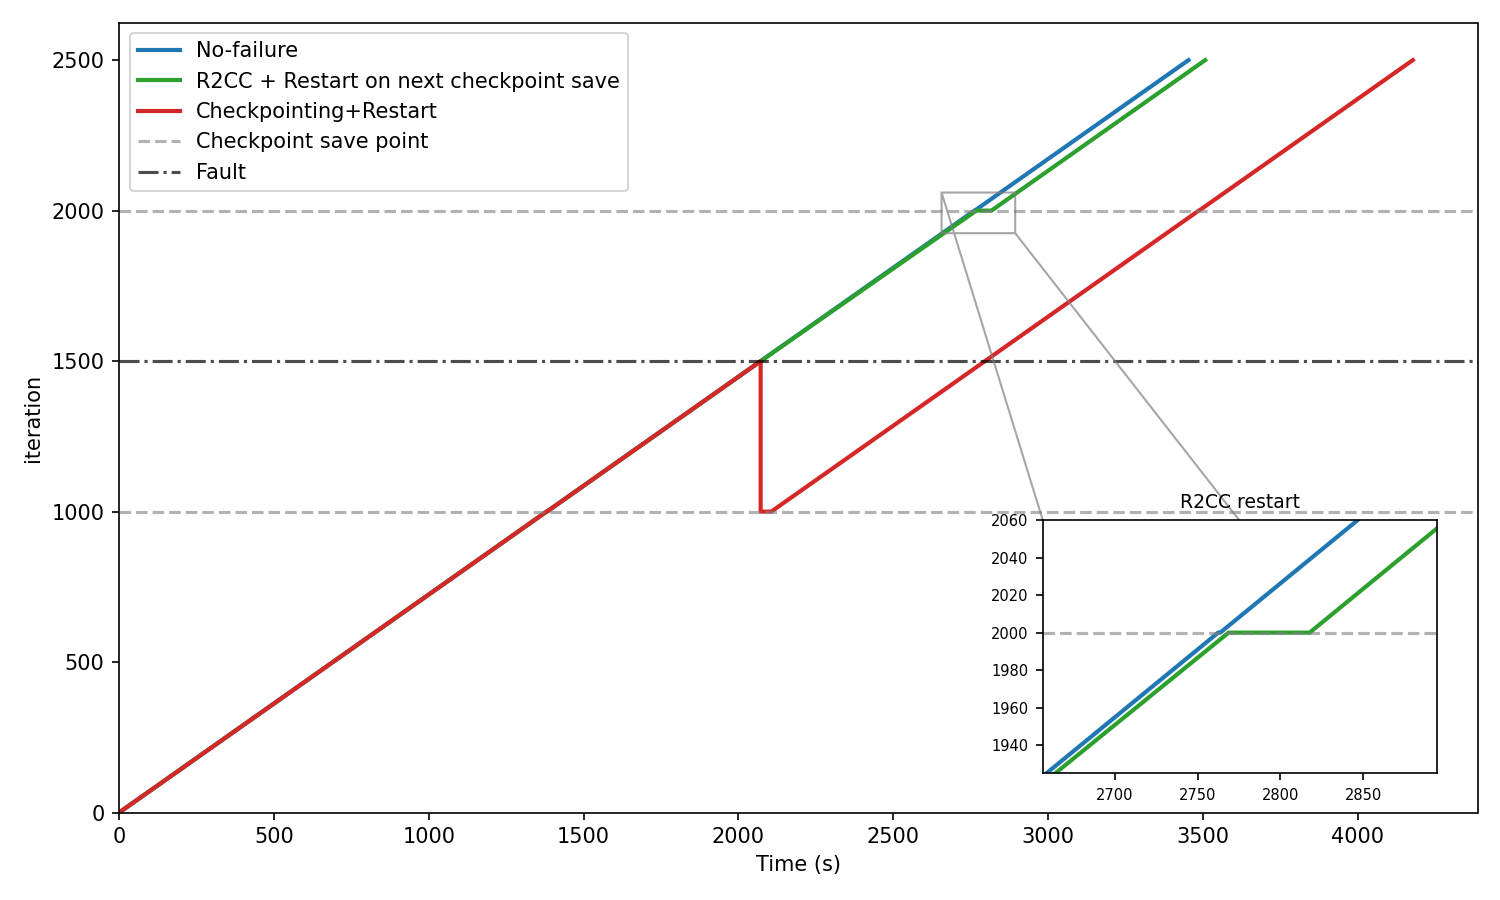
\includegraphics[width=0.7\columnwidth]{figs/section8/ckpt_recovery_dp32_x1000_fail1500_inset.png}
    \tightcaption{\textbf{Checkpoint and restore in a training workload}}
    \label{fig:checkpoint-and-restore}
\end{figure}
\section{Checkpoint and restore}\label{appendix:checkpoint}
Figure \ref{fig:checkpoint-and-restore} shows a training run with a NIC failure injected mid-interval between two checkpoints. The naive baseline aborts at the failure and rolls back to the previous checkpoint, discarding the iterations since the last save; R2CC keeps training through to the next scheduled checkpoint, saves state, and only then restarts to recover the NIC, resuming without losing progress.

\section{Training Quality Under a NIC Failure}\label{app:quality}
\paragraph{Setup.} We train GPT-2 (124M)~\cite{radford2019language} on WikiText-103~\cite{merity2016pointer} with PyTorch DDP for 1,000 updates on three CloudLab servers, each with two V100S GPUs and three NIC ports. After update 400, we install a drop rule on one NIC port of one server for the rest of the run, leaving the other NICs up. Runs are deterministic, and each failure run is paired with a failure-free run of the same seed (three seeds per policy).

\paragraph{Results.} Without failures, R2CC is bit-identical to the upstream NCCL 2.23.4 it forks from: the same losses and the same hashes of reduced gradients and parameters at every checked update. Under the failure, R2CC completes the interrupted AllReduce on the backup connection and continues under R2CC-Balance or R2CC-AllReduce without restart or rollback. HotRepair itself is lossless: the repaired collective at update 401 produces a bit-identical reduced gradient. Differences begin only at update 402, where R2CC-Balance and R2CC-AllReduce redistribute data across the remaining NICs and thereby change the order in which gradients are summed; floating-point addition is not associative, so a different order rounds differently. To verify that reordering is the only effect, we re-sum the recorded gradient inputs in double precision as an exact reference: both NCCL's and R2CC's results stay within a relative error of $5.8\times10^{-8}$ of it, i.e., ordinary FP32 rounding. Figure~\ref{fig:quality} shows the paired trajectories: the per-update loss deviation stays within $2.4\times10^{-3}$ nats/token with no consistent sign, and final test perplexity rises by at most 0.023\% (Table~\ref{tab:quality}).

\begin{figure}[t]
    \centering
    \begin{subfigure}[b]{0.48\columnwidth}
        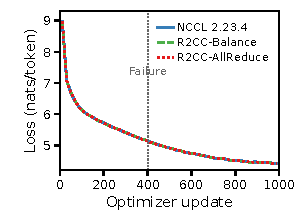
\includegraphics[width=\textwidth]{figs/appendix/appendix_loss.pdf}
        \caption{Training loss trajectory.}
        \label{fig:loss-traj}
    \end{subfigure}
    \hfill
    \begin{subfigure}[b]{0.48\columnwidth}
        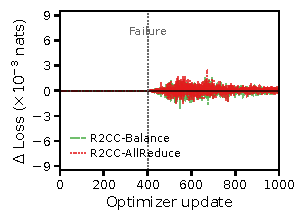
\includegraphics[width=\textwidth]{figs/appendix/appendix_deviation.pdf}
        \caption{Training loss deviation.}
        \label{fig:loss-dev}
    \end{subfigure}
    \tightcaption{Training loss under a persistent NIC-port failure (GPT-2 124M, WikiText-103, 3 seeds).}
    \label{fig:quality}
\end{figure}

\begin{table}[h]
\centering
\small
\begin{tabular}{lrr}
\toprule
Condition & Test PPL & Max.\ paired $\Delta$ \\
\midrule
NCCL 2.23.4, no failure & 76.085 & -- \\
R2CC, no failure & 76.085 & $0.000\%$ \\
R2CC-Balance, failure & 76.085 & $+0.008\%$ \\
R2CC-AllReduce, failure & 76.086 & $+0.023\%$ \\
\bottomrule
\end{tabular}
\caption{Final test perplexity (mean of three seeds). $\Delta$ is the worst-case increase over the NCCL baseline run with the same seed.}
\label{tab:quality}
\end{table}

\section{Discussion}\label{app:discussion}
\paragraph{Multi-plane fabrics and direct-attached NICs.} Multi-plane fabrics connect each NIC to several independent switch planes, so a link or switch failure in one plane is masked at reduced bandwidth. The affected NIC then runs slower than its peers, and R2CC's schedule optimization could further rebalance traffic toward the other NICs once the fabric exposes this reduced bandwidth. A fault in the NIC itself, such as a hardware, firmware, or PCIe error, still takes down all of its planes, and R2CC handles it by failing over to another NIC. In GPU servers that attach each NIC directly to its GPU, such as HGX B300, a GPU has no direct PCIe path to the NICs of other GPUs, but when its NIC fails, R2CC can still relay its traffic over NVLink to GPUs with healthy NICs through PXN.

\paragraph{SHARP.} NVLink SHARP performs reductions inside the NVSwitch without traversing NICs, so it is complementary to R2CC, which protects inter-node transfers. InfiniBand SHARP instead keeps partial aggregates in switch memory, so a NIC failure during an in-network reduction cannot be repaired by migrating connections, and R2CC does not currently handle it. Supporting SHARP, e.g., by falling back to the host-based path or redistributing data across the aggregation trees of the surviving rails, is left to future work.

\paragraph{CUDA Graphs.} R2CC is compatible with CUDA Graphs. Hot repair only changes which connection the CPU proxy uses, and NCCL re-drives the proxy on every replay, so a graph captured before a failure keeps replaying over the backup NIC with its captured kernels and buffer addresses unchanged. The schedule optimizations of \S\ref{sec:single-failure} are decided when a collective is enqueued, so they take effect once the framework re-captures the graph, e.g., upon R2CC's degradation signal (\S\ref{sec:signal-restore}). A large graph does not need to be re-captured as a whole, since only the child graph that holds the collective has to be re-captured and swapped in. Re-capture only records operations without executing them, so capturing and instantiating a graph containing the collective takes about one to two milliseconds, and the next replay already runs the new schedule. R2CC-AllReduce must create its sub-communicators outside capture, so it needs one eager collective after repair, which adds a one-time setup of about 0.3\,s to a regular iteration. Table~\ref{tab:cuda-graphs} shows these behaviors on a three-server CloudLab testbed.

\begin{table}[t]
\centering
\small
\begin{tabular}{lrr}
\toprule
 & Time & Re-capture \\
Replayed graph (4\,GiB AllReduce) & / iter & overhead$^{*}$ \\
\midrule
Pre-failure graph, healthy & 2.03\,s & -- \\
Pre-failure graph, HotRepair & 4.07\,s & -- \\
Re-captured as R2CC-Balance & 3.04\,s & 1.7\,ms \\
Re-captured as R2CC-AllReduce & 2.79\,s & 0.33\,s \\
\bottomrule
\end{tabular}
\caption{CUDA Graphs on three CloudLab servers, each with two V100S GPUs and three NIC ports limited to 10\,Gbps. $^{*}$Re-capture overhead is the time of the iteration that performs the re-capture, including the eager collective that R2CC-AllReduce needs to create its sub-communicators, minus the time of an iteration replayed from the new graph.}
\label{tab:cuda-graphs}
\end{table}
